\chapter{Methodology}
\section{Software Development Approach}
Agile development is a software development approach that emphasizes incremental progress and rapid cycles. It involves releasing small increments of functionality that build upon previous versions. Thorough testing is conducted for each release to ensure software quality. Agile is often employed for time-critical applications. Although this project is not time-critical this model seems to be the most optimal and practical in our case.
\begin{figure}[hbt!]
    \center{
        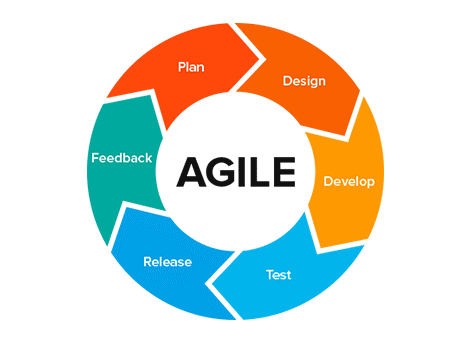
\includegraphics[width=0.75\textwidth]{./img/agile.png}
        \caption{Agile Model for Software Development}
        \subcaption*{\textit{source: \textcolor{blue}{https://mobilelive.medium.com/agile-development-a-comprehensive-guide-for-the-modern-era-d2fe9ae7b395}}}
    }
\end{figure}
\newpage
\section{Proposed System Block Diagram}
    \begin{figure}[hbt!]
    \center{
        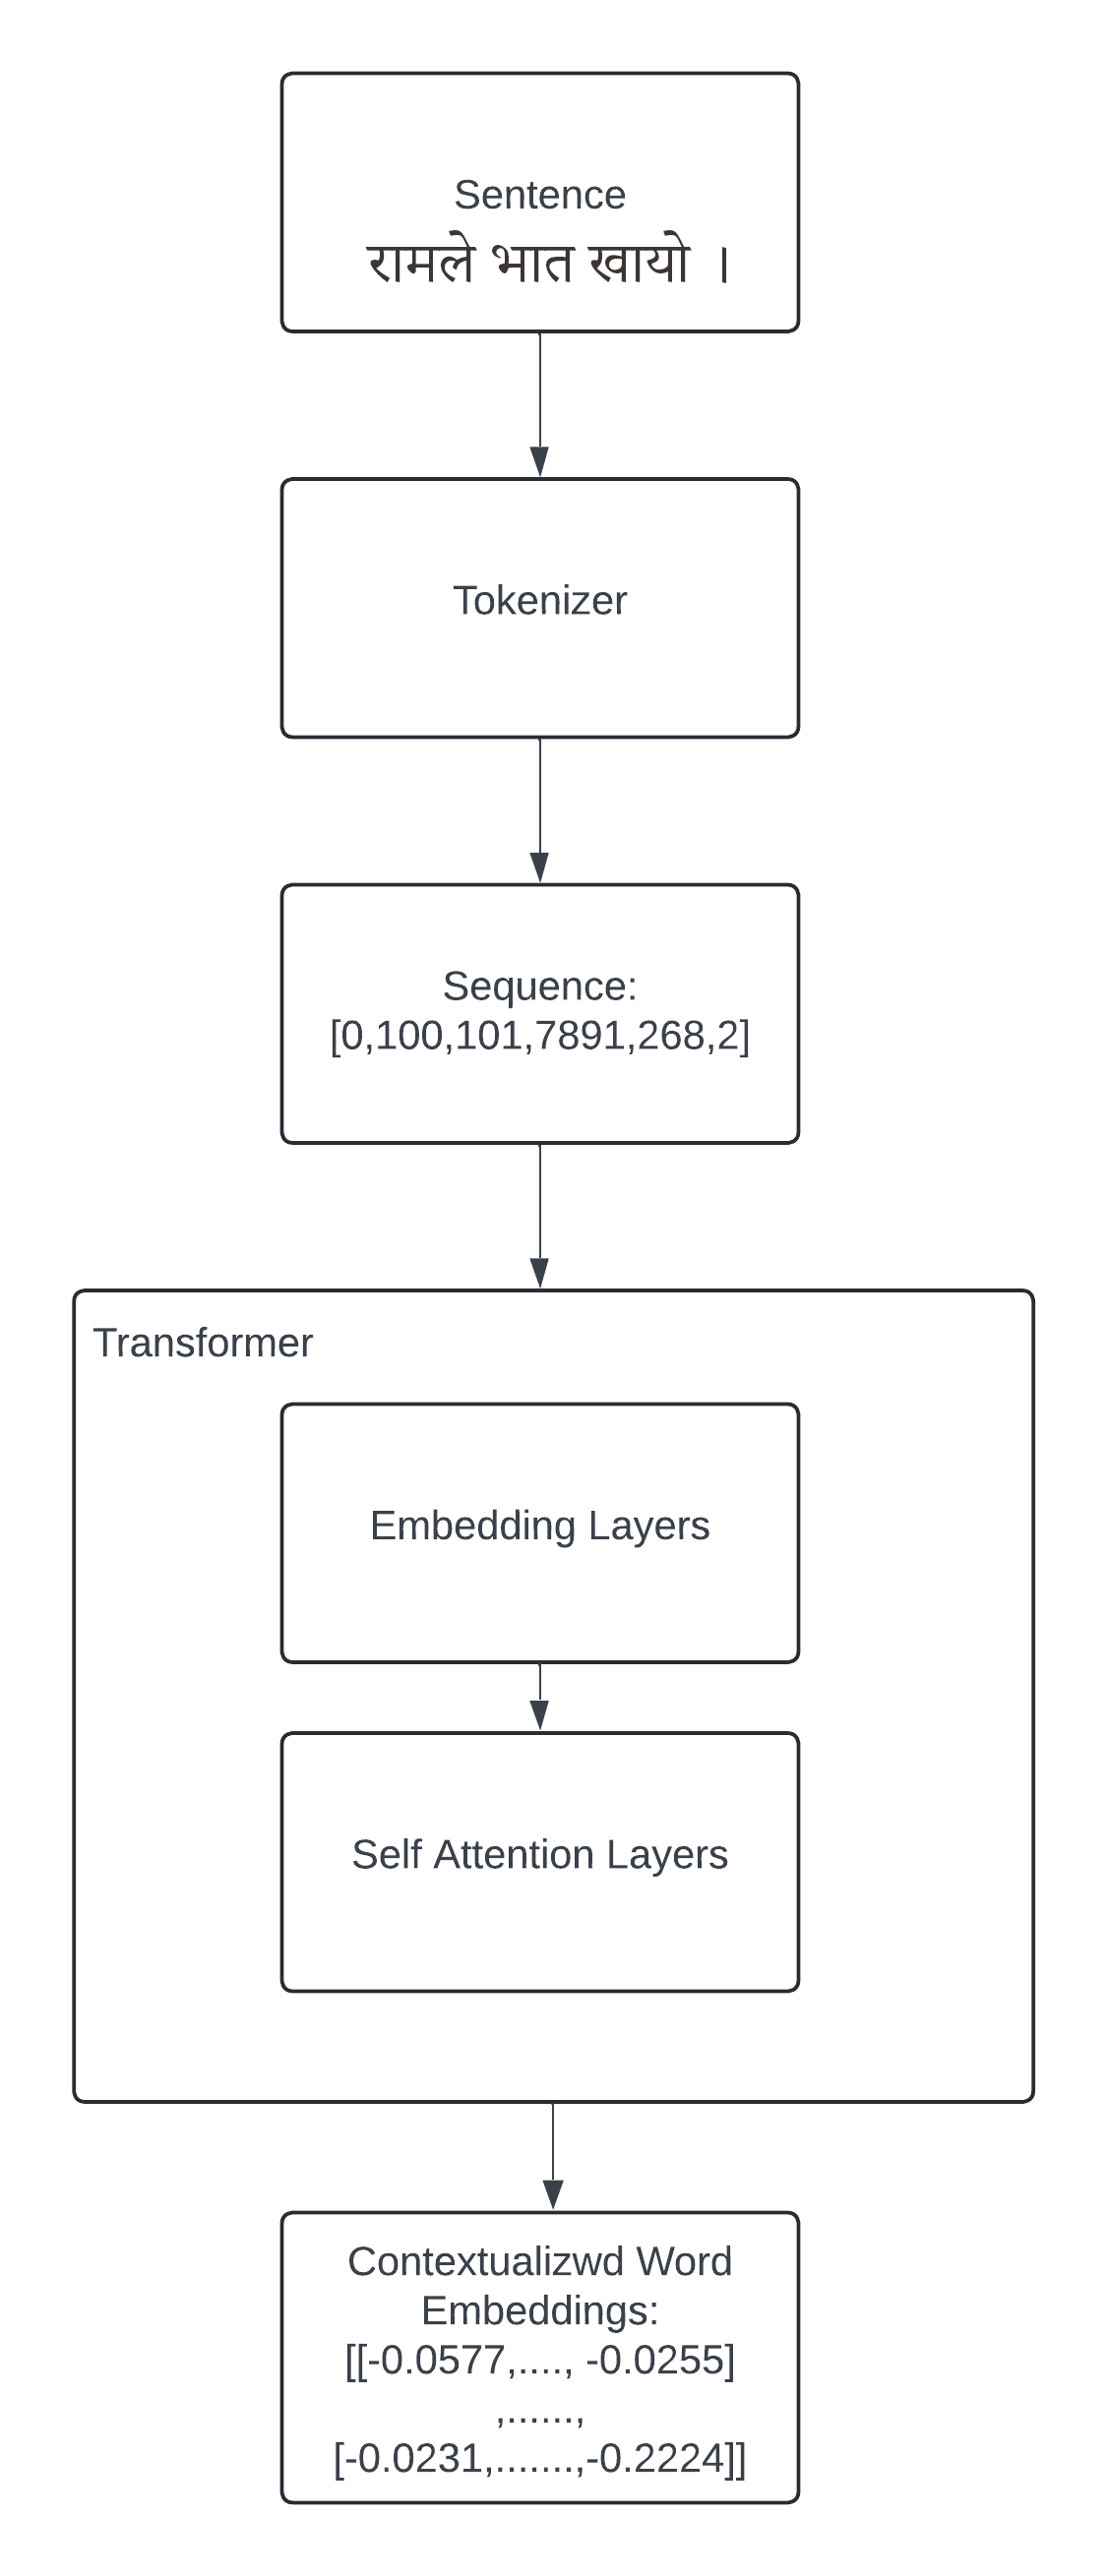
\includegraphics[width=0.6\textwidth]{./img/Block_Diagram.png}
        \caption{Block diagram of Proposed Sytem}
        }
    \end{figure}

\section{Description of Working Flow of Proposed System}
\begin{enumerate}
    \item \textbf{Sentence Input}:
    \begin{itemize}
        \item The process starts with a given sentence in the Nepali language: \textsanskrit{रामले भात खायो}
    \end{itemize}
    
    \item \textbf{Tokenizer}:
    \begin{itemize}
        \item The sentence is passed to a tokenizer, which breaks down the sentence into individual tokens. The tokens are then converted into a sequence of numerical IDs. For example, the sentence \textsanskrit{रामले भात खायो} is converted into the sequence \texttt{[0, 100, 101, 7891, 268, 2]}.
    \end{itemize}
    
    \item \textbf{Transformer Model}:
    \begin{itemize}
        \item The tokenized sequence is then fed into a Transformer model, which consists of several layers. This model processes the sequence to generate contextualized word embeddings.
        
        \begin{itemize}
            \item \textbf{Embedding Layers}:
            \begin{itemize}
                \item The first part of the Transformer model is the embedding layers. These layers convert the input token IDs into dense vectors of fixed size. These vectors capture semantic information about the words.
            \end{itemize}
            
            \item \textbf{Self-Attention Layers}:
            \begin{itemize}
                \item After the embedding layers, the vectors pass through multiple self-attention layers. These layers allow the model to weigh the importance of different words in the sentence relative to each other, thereby capturing the context of each word in relation to the entire sentence.
            \end{itemize}
        \end{itemize}
    \end{itemize}
    
    \item \textbf{Contextualized Word Embeddings Output}:
    \begin{itemize}
        \item The final output of the Transformer model is a set of contextualized word embeddings. Each word in the input sentence is now represented by a vector that encodes both its meaning and its context within the sentence. For example, the embeddings might look like:
        [[-0.0577, ..., -0.0255],
         ...,
         [-0.0231, ..., -0.2224]].
    \end{itemize}
\end{enumerate}

% \section{Performance Evaluation Metrics}
